\documentclass[12pt]{article}
\usepackage[a4paper, total={6in, 10in}]{geometry}

\usepackage{graphicx}
\usepackage{abstract}
\usepackage{hyperref}
\usepackage{listings}
\usepackage{indentfirst}
\usepackage{amssymb}
\usepackage{titling}
\usepackage{mwe}
\usepackage{fancyhdr}
\usepackage{setspace}

\graphicspath{ {./images/} }
\onehalfspacing

\setlength{\parskip}{3mm}   % Add space between paragraphs.
\setlength{\parindent}{0.5in}
\setlength{\droptitle}{-35pt}

\fancypagestyle{plain}{
    \vspace{3ex}
    \fancyhead[L]{November 14th, 2020}
    \renewcommand{\headrulewidth}{0.5pt}
}

\pretitle{\begin{center} \LARGE \textbf}
\posttitle{\end{center} \vspace{-3ex}}
\preauthor{\begin{center} \large}
\postauthor{\end{center} \vspace{-3ex}}
\predate{\begin{center} \small \emph}
\postdate{\end{center} \vspace{-3ex}}

\title{Chapter 6 Summary \& Review Questions}
\author{Chris Nutter\thanks{Dedicated to @QuesoGrande a.k.a. Jared D.}}
\date{CPSC 315}

% --> Here we go, satellite radio, y'all get hit with a...

\begin{document}
\maketitle

%\begin{center} \vspace{-4ex}|\vspace{-3ex} \end{center}
\normalsize

\tableofcontents    
\vspace{4ex}

\begin{center} Content begins on next page. \end{center}

\newpage
\doublespacing
% --> First Chapter

\section{Chapter 6 Summary}
    \indent Cyber Security is very important to maintaining and preserving our information. The government is in place to protect and serve its citizens to the best of their ability. However the government also makes a living off of its people and will tend to put policies in place to keep citizens in order. This is where governments will try to obtain information on people in order to "protect" other people. Government systems on all level have their benefits and disadvantages. The federal government is in charge of all states and puts nationwide policies into effect while the state government governs just the people within each state. Why this is important is due to how cyber security practices go per state.\\
    \indent Personally the federal government shouldn't have a lot of power because this allows too much constriction to rules. If a policy is put into place in a state and I don't agree with it, I can branch away from that state while federal policies are nationwide. Security practices that are federally run ted to be very unsafe towards the community. Acts like the Patriot Act that allows surveillance to be done in order to protect foreign attacks. While the meaning is good, the execution is very unsafe towards its citizens.\\
    \indent 9/11 was a major hit towards the United States and it brought on this new idea of are we really safe. Physically and technology-wise. Many federal agencies were caught illegally obtaining information in order to better "understand 9/11 and why it happened." (This is not a direct quote but more of an exaggeration of what I presume their intentions were)
\newpage
\onehalfspacing

\section{Review Questions}
    \begin{enumerate}
        \item Privacy is considered by these men to be a human right. They all each have very similar ideas of everyone else and yourself. Privacy being how much everyone knows about me.
        \item Wiretapping was a felony case in 1879 but was used by the NYC police until 1920. After World War II, FBI director J. Edgar Hoover pressed to have the ban on wiretapping withdrawn. The NSA were also caught wiretapping after 9/11 trying to obtain information about al-Qaeda.
        \item COPPA is a huge benefit for children as it protects children online who aren't old enough to understand. California's Reader Privacy Act was passed in 2011 which prohibits commercial provider of book service to disclose information from subjects. Health Information Technology for Economic and Clinical Health Act protects patients from unwanted information to be sold about medical records.
        \item The US Census is important as it gives our government a way to understand how things should be put into effect. Voting is a huge achievement as it allows our country to speak about who they want in charge. 
        \item Three examples of government agencies illegally obtaining information is NSA wiretapping phones post-9/11, the NYC police wiretapping even after being placed as a felony. 
        \item Telephony metadata is the collection of cellphone records done by the government as a way to keep tabs on its citizens post-9/11. Once the NSA were caught obtaining information, people were not happy to learn about the government spying on them.
        \item All operations involved the tampering and wiretapping of information from third-parties. Not all these were successful however as some were done illegally (i.e NSA wiretapping).
        \item They let their ISP handle their emails but they're also able to investigate the email as well giving them control over your information which could be done in bad practice.
        \item The use of National Security Letters can raise privacy concerns as it gives the government a way to spy on its citizens.
        \item The five tenets are:
        \begin{enumerate}
            \item No secret information.
            \item Citizens must know what information they are storing.
            \item People can opt-out of information if they choose to.
            \item People can change any errors written.
            \item Make sure the information is secure.
        \end{enumerate}
        \item The Privacy Act didn't particularly help anything as it just allowed the government to keep the tabs on people not the organizations.
        \item Only certain information is kept for a certain amount of time. Which can allow companies to make judgements.
        \item The government can collect our information like medical records for example and use that to send us ads for government-based healthcare plans, different tax brackets, or even avoid us from being able to do things other people can (i.e driving a car).
        \item You only have one social security number linked to a person so it shouldn't be used everyone and for everything.
        \item National identification card allows people to distinguish who they are and it also lets people use something that isn't hugely private. The problem however is this ID can be stolen or worse even used against you in identity fraud.
        \item The government has mandated how companies can collect information especially websites requiring user verification. The government has helped the illegal use of your information by making it required where your information is used. The government has made it a felony to invade people's privacy and illegally obtain their information. 
    \end{enumerate}

\end{document} 

% Possibly Important LaTeX Functions %
% ================================== %

%   \begin{figure}[hbtp]
%       \centering
%       \fbox{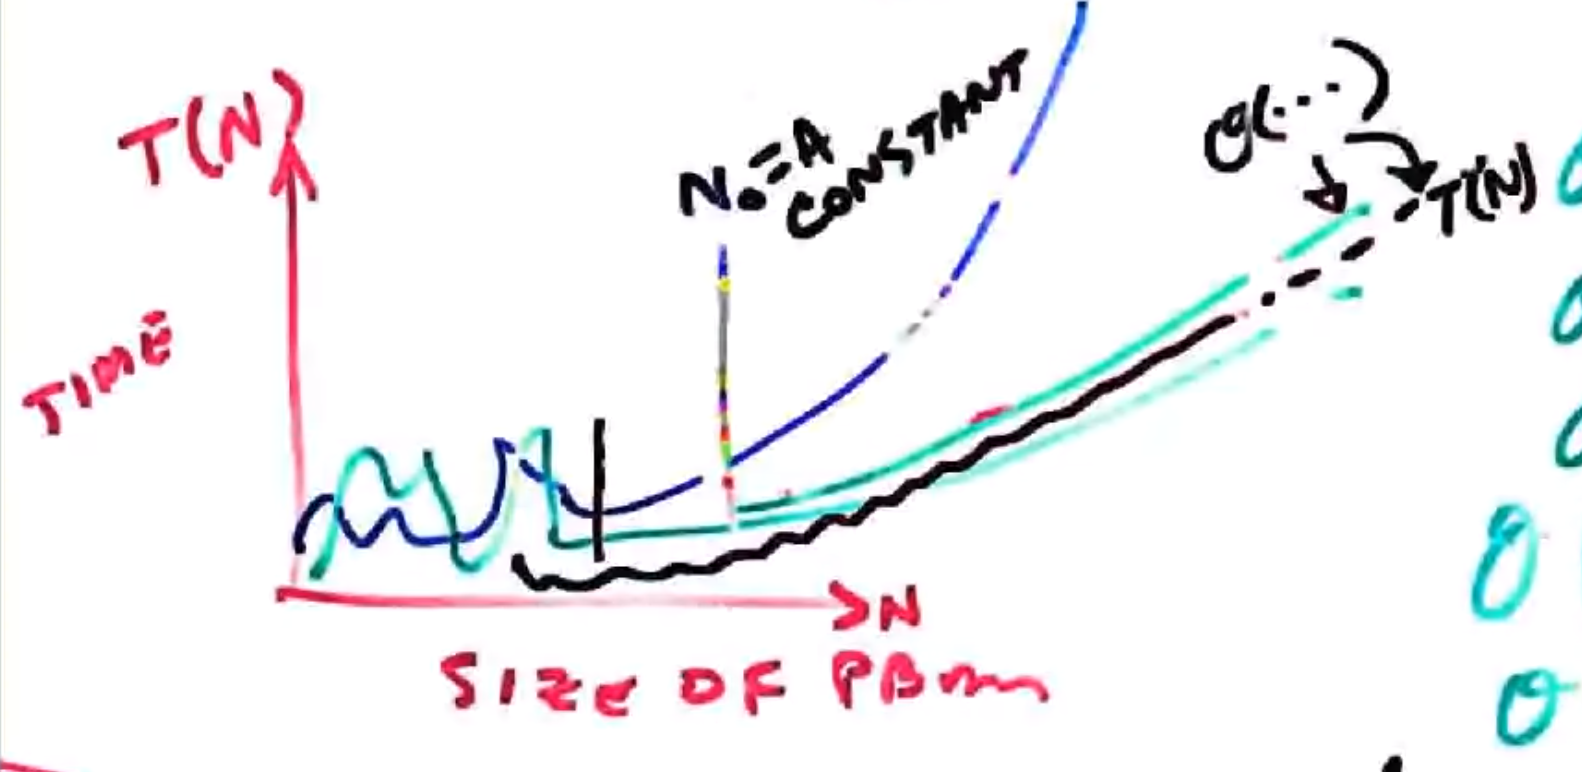
\includegraphics[width=13.8cm]{big_o.png}}
%       \caption{Big(O) Notation}
%   \end{figure}

%   \begin{lstlisting}[language=Python] 
%        print('hello world') 
%   \end{lstlisting}  

